\documentclass[10pt,a4paper]{article}
\usepackage[utf8]{inputenc}
\usepackage[T1]{fontenc}
\usepackage[romanian]{babel}
\usepackage[margin=1.7cm]{geometry}
\usepackage{amsmath,amssymb,mathtools}
\usepackage{enumitem}
\usepackage{titlesec}
\usepackage{parskip}
\usepackage{tikz}
\usetikzlibrary{calc,arrows.meta,positioning}
\usepackage{pgfplots}
\pgfplotsset{compat=1.18}
\usepackage[most]{tcolorbox}
\usepackage{xcolor}

\newtcolorbox{res}{colback=red!6,colframe=red!65!black,boxrule=0.6pt,arc=1.5pt,
  left=4pt,right=4pt,top=2pt,bottom=2pt,breakable}
\newtcolorbox{chk}{colback=green!6,colframe=green!45!black,boxrule=0.6pt,arc=1.5pt,
  left=4pt,right=4pt,top=2pt,bottom=2pt,breakable}

\setlist{nosep, topsep=2pt, itemsep=2pt, leftmargin=1.3em}
\titlespacing*{\section}{0pt}{6pt}{2pt}
\titlespacing*{\subsection}{0pt}{4pt}{1pt}
\renewcommand{\baselinestretch}{0.96}
\setlength{\parindent}{0pt}
\pagestyle{empty}

\begin{document}
\begin{center}
{\large\bfseries Rezolvare --- Bilet de examen SAE, sesiunea toamn\u{a} 2026}
\end{center}
\vspace{-0.2cm}

\section*{1. $G(s)=\dfrac{9}{s(s+3)}$, $T_e=1$s}

\subsection*{a) $H(z)$ -- metoda trapezului (Tustin)}
$$\textcolor{blue}{s=\frac2{T_e}\cdot\frac{z-1}{z+1}=2\,\frac{z-1}{z+1}}\qquad s+3=\frac{2(z-1)+3(z+1)}{z+1}=\frac{5z+1}{z+1}$$
$$G(z)=\frac9{s(s+3)}=\frac{9(z+1)^2}{2(z-1)(5z+1)}=\frac{9z^2+18z+9}{10z^2-8z-2}$$
$$H(z)=\frac{G(z)}{1+G(z)}=\frac{9z^2+18z+9}{(10z^2-8z-2)+(9z^2+18z+9)}$$
\begin{res}
$$H(z)=\frac{9z^2+18z+9}{19z^2+10z+7}$$
\end{res}

\subsection*{b) $G(z)$ -- ecuația cu diferențe}
$$G(s)=\frac9{s(s+3)}\ \Rightarrow\ \ddot y+3\dot y=9u$$
$$\color{blue}\dot y\approx\frac{y[k]-y[k-1]}{T_e}=y[k]-y[k-1]\qquad
\ddot y\approx\frac{y[k]-2y[k-1]+y[k-2]}{T_e^2}=y[k]-2y[k-1]+y[k-2]$$
$$\big(y[k]-2y[k-1]+y[k-2]\big)+3\big(y[k]-y[k-1]\big)=9u[k]$$
\begin{res}
$$4y[k]-5y[k-1]+y[k-2]=9u[k]$$
\end{res}
$$q^{-1}y[k]=y[k-1]:\qquad \big(4-5q^{-1}+q^{-2}\big)y[k]=9u[k]\ \Rightarrow\ G(q)=\frac9{4-5q^{-1}+q^{-2}}\ \overset{q\to z}{\Rightarrow}$$
\begin{res}
$$G(z)=\frac{9z^2}{4z^2-5z+1}=\frac{9z^2}{(z-1)(4z-1)}$$
\end{res}

\subsection*{c) Eroare staționară}
$$G(z)=\frac{9(z+1)^2}{2(z-1)(5z+1)}$$
$$K_p=\lim_{z\to1}G(z)=\infty$$
$$K_v=\frac1{T_e}\lim_{z\to1}(z-1)\,G(z)=\lim_{z\to1}(z-1)\cdot\frac{9(z+1)^2}{2(z-1)(5z+1)}=\lim_{z\to1}\frac{9(z+1)^2}{2(5z+1)}=\frac{9\cdot4}{2\cdot6}=\frac{36}{12}=3$$
$$K_a=\frac1{T_e^2}\lim_{z\to1}(z-1)^2G(z)=\lim_{z\to1}(z-1)\cdot\frac{9(z+1)^2}{2(5z+1)}=0$$
\begin{res}
$$e_{ss}(\text{treaptă})=\frac1{1+K_p}=0\qquad
e_{ss}(\text{rampă})=\frac1{K_v}=\frac13\approx0.33\qquad
e_{ss}(\text{parabolă})=\frac1{K_a}=\infty$$
\end{res}

\subsection*{d) Răspuns la treaptă unitară ($\mathcal Z^{-1}$)}
$$H(z)=\frac{Y(z)}{R(z)}=\frac{9z^2+18z+9}{19z^2+10z+7}\qquad\Rightarrow\qquad Y(z)=H(z)\cdot R(z)$$
$$\color{blue}R(z)=\frac{z}{z-1}$$
$$Y(z)=\underbrace{\frac{9z^2+18z+9}{19z^2+10z+7}}_{H(z)}\cdot\underbrace{\frac{z}{z-1}}_{R(z)}=\frac{(9z^2+18z+9)\cdot z}{(19z^2+10z+7)\cdot(z-1)}$$
$$Y(z)=\frac{z(9z^2+18z+9)}{(z-1)(19z^2+10z+7)}$$
$$z_{1,2}=\frac{-10\pm\sqrt{100-4\cdot19\cdot7}}{38}=-0.26\pm j0.55=\alpha\pm j\beta=r\,e^{\pm j\theta}$$
$$r=|z_{1,2}|=\sqrt{\alpha^2+\beta^2}=\sqrt{7/19}=0.61$$
$$\theta=\arg z_{1,2}=180^\circ-\arctan\frac{\beta}{|\alpha|}$$
$$\theta=180^\circ-\arctan\frac{0.55}{0.26}=180^\circ-\arctan(2.08)=180^\circ-64.31^\circ$$
$$\theta=115.69^\circ$$
$$\frac{Y(z)}z=\frac{9z^2+18z+9}{(z-1)(19z^2+10z+7)}=\frac{A}{z-1}+\frac{Bz+C}{19z^2+10z+7}$$
$$9z^2+18z+9=A(19z^2+10z+7)+(Bz+C)(z-1)$$
$$z=1:\ 36=36A\Rightarrow A=1\qquad \text{coef. }z^2:\ 19A+B=9\Rightarrow B=-10\qquad \text{termen liber}:\ 7A-C=9\Rightarrow C=-2$$
$$19z^2+10z+7=19(z-z_1)(z-z_2)=19\big[z-(\alpha{+}j\beta)\big]\big[z-(\alpha{-}j\beta)\big]$$
$$=19\big[(z-\alpha)^2-(j\beta)^2\big]=19\big[(z-\alpha)^2+\beta^2\big]=19\big[z^2-2\alpha z+\underbrace{\alpha^2+\beta^2}_{r^2}\big]$$
$$19z^2+10z+7=19\big(z^2-2rz\cos\theta+r^2\big),\quad r\cos\theta=\alpha=-0.26,\ r\sin\theta=\beta=0.55$$
$$\color{blue}\mathcal Z\{r^k\cos k\theta\}=\frac{z(z-r\cos\theta)}{z^2-2rz\cos\theta+r^2}\qquad \mathcal Z\{r^k\sin k\theta\}=\frac{zr\sin\theta}{z^2-2rz\cos\theta+r^2}$$
$$Y(z)=\frac{z}{z-1}+\frac{z(Bz+C)}{19\big(z^2-2rz\cos\theta+r^2\big)}$$
$$Bz+C=B(z-r\cos\theta)+\underbrace{\big[B\,r\cos\theta+C\big]}_{D}$$
$$D=B\,r\cos\theta+C=(-10)(-0.26)+(-2)=2.63-2=0.63$$
$$\frac{z(Bz+C)}{19(z^2-2rz\cos\theta+r^2)}=\frac{B}{19}\cdot\frac{z(z-r\cos\theta)}{z^2-2rz\cos\theta+r^2}+\frac{D}{19}\cdot\frac{z}{z^2-2rz\cos\theta+r^2}$$
$$\frac{B}{19}=\frac{-10}{19}=-0.53$$
$$\frac D{19}\,z=\frac{D}{19\,r\sin\theta}\cdot(z\,r\sin\theta)$$
$$\frac{D}{19\,r\sin\theta}=\frac{0.63}{19\cdot0.55}=\frac{0.63}{10.39}=0.06$$
$$Y(z)=\frac z{z-1}\underbrace{-0.53}_{B/19}\,\frac{z(z-r\cos\theta)}{z^2-2rz\cos\theta+r^2}+\underbrace{0.06}_{D/(19\,r\sin\theta)}\,\frac{z\,r\sin\theta}{z^2-2rz\cos\theta+r^2}$$
\begin{res}
$$y(k)=1-0.53\,r^k\cos(k\theta)+0.06\,r^k\sin(k\theta),\qquad k\ge0$$
\end{res}
\begin{center}
\begin{tabular}{@{}rrrrrrrrrrrr@{}}
$k$&0&1&2&3&4&5&6&7&8&9&10\\
$y(k)$&0.47&1.17&1.10&0.88&1.02&1.03&0.97&1.00&1.01&0.99&1.00\\
\end{tabular}
\end{center}

\begin{center}
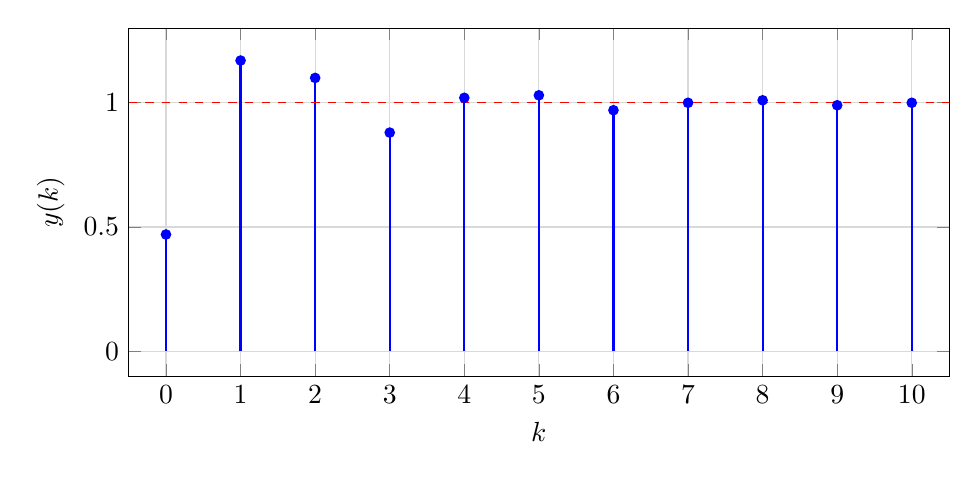
\begin{tikzpicture}
\begin{axis}[
  width=12cm,height=6cm,
  xlabel={$k$}, ylabel={$y(k)$},
  xmin=-0.5,xmax=10.5, ymin=-0.1, ymax=1.3,
  grid=both, minor grid style={gray!15}, major grid style={gray!30},
]
\addplot[ycomb,thick,blue,mark=*,mark size=1.5pt,mark options={fill=blue}] coordinates {
(0,0.47) (1,1.17) (2,1.10) (3,0.88) (4,1.02) (5,1.03) (6,0.97) (7,1.00)
(8,1.01) (9,0.99) (10,1.00)
};
\addplot[red,dashed,domain=-0.5:10.5] {1};
\end{axis}
\end{tikzpicture}
\end{center}

\subsection*{e) Caracteristici de frecvență (transformarea $w$)}
$$\color{blue}z=\frac{1+\frac{T_e}2w}{1-\frac{T_e}2w}\overset{T_e=1}{=}\frac{1+0.5w}{1-0.5w}=\frac ND,\quad N=1+0.5w,\ D=1-0.5w\ \Rightarrow\ z+1=\frac2D$$
$$H(z)=\frac{9(z+1)^2}{19z^2+10z+7}\qquad
9(z+1)^2=\frac{36}{D^2}\qquad
19z^2+10z+7=\frac{19N^2+10ND+7D^2}{D^2}=\frac{4w^2+12w+36}{D^2}$$
\begin{res}
$$H(w)=\frac{36}{4w^2+12w+36}=\frac9{w^2+3w+9}$$
\end{res}
$$H(w)=\frac9{w^2+3w+9}=\frac1{1+\frac13w+\frac19w^2}\ \overset{!}{=}\ \textcolor{blue}{\frac{K}{1+2\alpha Tw+T^2w^2}}$$
$$\text{termen liber: }\ 1=K\ \Rightarrow\ K=1$$
$$\text{coef. }w^2:\ T^2=\frac19\ \Rightarrow\ T=\frac13$$
$$\text{coef. }w:\ 2\alpha T=\frac13\ \Rightarrow\ \alpha=\frac1{2T}\cdot\frac13=\frac1{2\cdot\frac13}\cdot\frac13=\frac12$$
\begin{res}
$$T=\frac13=0.33\text{ s}\qquad \alpha=0.5\qquad K=1\Rightarrow K_{dB}=0\text{ dB}\qquad \omega_f=\frac1T=3\text{ rad/s}$$
\end{res}
\begin{itemize}
\item amplitudine: $K_{dB}=0$ dB pentru $\omega<\omega_f$; pantă $-40$dB/decadă pentru $\omega>\omega_f$; frângere $(\omega_f,K_{dB})=(3,0)$.
\item fază: $0^\circ$ pentru $\omega<\omega_f/10=0.3$; dreaptă (în $\lg\omega$) până la $-180^\circ$ la $10\omega_f=30$; $-90^\circ$ la $\omega=\omega_f=3$.
\end{itemize}

\begin{center}
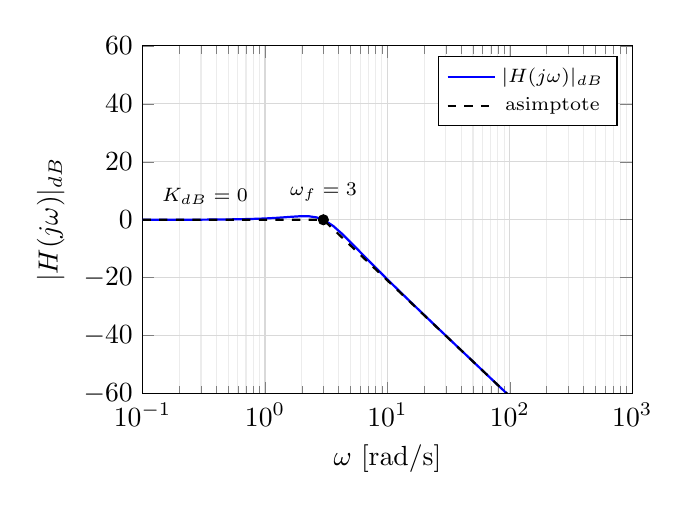
\begin{tikzpicture}
\begin{semilogxaxis}[
  width=7.8cm,height=6cm,
  xlabel={$\omega$ [rad/s]}, ylabel={$|H(j\omega)|_{dB}$},
  xmin=0.1,xmax=1000, ymin=-60,ymax=60,
  ytick={-60,-40,-20,0,20,40,60},
  grid=both, minor grid style={gray!15}, major grid style={gray!30},
  legend style={font=\scriptsize,at={(0.97,0.97)},anchor=north east},
]
\addplot[blue,thick] coordinates {
(0.1,0.01) (0.12,0.01) (0.14,0.01) (0.16,0.01) (0.19,0.02) (0.22,0.02) (0.26,0.03) (0.30,0.04) (0.35,0.06) (0.41,0.08) (0.48,0.11) (0.56,0.15) (0.65,0.20) (0.76,0.27) (0.89,0.36) (1.04,0.48) (1.22,0.64) (1.42,0.83) (1.66,1.04) (1.94,1.21) (2.27,1.22) (2.65,0.81) (3.10,-0.31) (3.63,-2.23) (4.24,-4.75) (4.95,-7.56) (5.79,-10.47) (6.77,-13.39) (7.91,-16.28) (9.25,-19.13) (10.81,-21.95) (12.64,-24.75) (14.77,-27.52) (17.27,-30.28) (20.19,-33.02) (23.60,-35.76) (27.59,-38.49) (32.25,-41.22) (37.69,-43.94) (44.06,-46.66) (51.51,-49.38) (60.21,-52.09) (70.38,-54.81) (82.27,-57.52) (96.17,-60.23) (112.42,-62.95) (131.41,-65.66) (153.62,-68.37) (179.57,-71.08) (209.91,-73.80) (245.38,-76.51) (286.83,-79.22) (335.29,-81.93) (391.94,-84.64) (458.16,-87.36) (535.57,-90.07) (626.05,-92.78) (731.82,-95.49) (855.47,-98.20) (1000,-100.92)
};
\addlegendentry{$|H(j\omega)|_{dB}$}
\addplot[black,dashed,thick] coordinates {(0.1,0) (3,0) (1000,-100.92)};
\addlegendentry{asimptote}
\addplot[only marks,mark=*,black,mark size=1.8pt] coordinates {(3,0)};
\node[above] at (axis cs:3,3) {\scriptsize $\omega_f=3$};
\node[anchor=west] at (axis cs:0.12,8) {\scriptsize $K_{dB}=0$};
\end{semilogxaxis}
\end{tikzpicture}
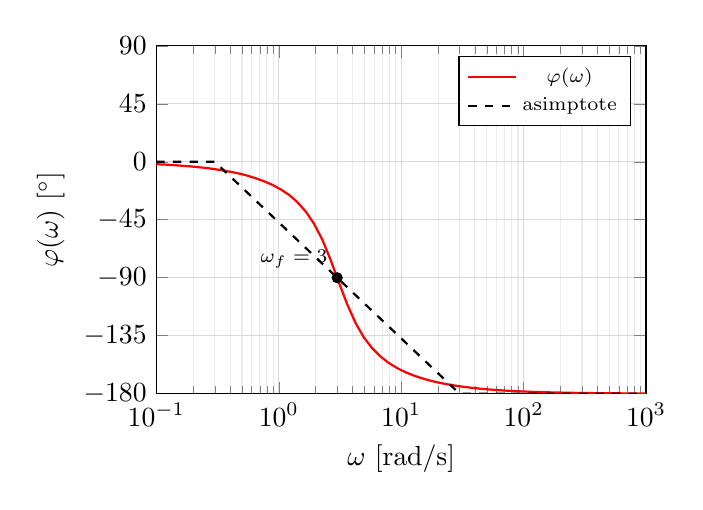
\begin{tikzpicture}
\begin{semilogxaxis}[
  width=7.8cm,height=6cm,
  xlabel={$\omega$ [rad/s]}, ylabel={$\varphi(\omega)$ [$^\circ$]},
  xmin=0.1,xmax=1000, ymin=-180,ymax=90,
  ytick={-180,-135,-90,-45,0,45,90},
  grid=both, minor grid style={gray!15}, major grid style={gray!30},
  legend style={font=\scriptsize,at={(0.97,0.97)},anchor=north east},
]
\addplot[red,thick] coordinates {
(0.1,-1.91) (0.12,-2.23) (0.14,-2.61) (0.16,-3.06) (0.19,-3.58) (0.22,-4.18) (0.26,-4.90) (0.30,-5.73) (0.35,-6.72) (0.41,-7.88) (0.48,-9.25) (0.56,-10.88) (0.65,-12.83) (0.76,-15.17) (0.89,-18.01) (1.04,-21.50) (1.22,-25.86) (1.42,-31.41) (1.66,-38.60) (1.94,-48.08) (2.27,-60.52) (2.65,-76.15) (3.10,-93.80) (3.63,-110.85) (4.24,-125.17) (4.95,-136.28) (5.79,-144.69) (6.77,-151.12) (7.91,-156.12) (9.25,-160.07) (10.81,-163.27) (12.64,-165.88) (14.77,-168.04) (17.27,-169.84) (20.19,-171.36) (23.60,-172.64) (27.59,-173.72) (32.25,-174.64) (37.69,-175.42) (44.06,-176.09) (51.51,-176.66) (60.21,-177.14) (70.38,-177.56) (82.27,-177.91) (96.17,-178.21) (112.42,-178.47) (131.41,-178.69) (153.62,-178.88) (179.57,-179.04) (209.91,-179.18) (245.38,-179.30) (286.83,-179.40) (335.29,-179.49) (391.94,-179.56) (458.16,-179.62) (535.57,-179.68) (626.05,-179.72) (731.82,-179.76) (855.47,-179.80) (1000,-179.83)
};
\addlegendentry{$\varphi(\omega)$}
\addplot[black,dashed,thick] coordinates {(0.1,0) (0.3,0) (30,-180) (1000,-180)};
\addlegendentry{asimptote}
\addplot[only marks,mark=*,black,mark size=1.8pt] coordinates {(3,-90)};
\node[above left] at (axis cs:3,-90) {\scriptsize $\omega_f=3$};
\end{semilogxaxis}
\end{tikzpicture}
\end{center}

\subsection*{f) Model cu variabile de stare}
$$H(z)=\frac{0.47z^2+0.95z+0.47}{z^2+0.53z+0.37}=\textcolor{blue}{D+\frac{b_1'z+b_0'}{z^2+a_1z+a_0}}$$
$$D=0.47\qquad b_1'=0.95-D\cdot0.53=0.70\qquad b_0'=0.47-D\cdot0.37=0.30$$
$$x_1(k+1)=x_2(k)\qquad x_2(k+1)=-0.37\,x_1(k)-0.53\,x_2(k)+r(k)$$
$$y(k)=0.30\,x_1(k)+0.70\,x_2(k)+0.47\,r(k)$$
\begin{res}
$$\Phi=\begin{pmatrix}0&1\\-0.37&-0.53\end{pmatrix},\quad \Gamma=\begin{pmatrix}0\\1\end{pmatrix},\quad C=\begin{pmatrix}0.30&0.70\end{pmatrix},\quad D=0.47$$
\end{res}
\begin{chk}
$$C(zI-\Phi)^{-1}\Gamma+D=\frac{0.47z^2+0.95z+0.47}{z^2+0.53z+0.37}=H(z)\ \checkmark$$
\end{chk}

\section*{2. $G_d(z)=\dfrac{0.37\,k\,(z+0.72)}{z^2-1.37z+0.37}$, $T_e=1$s}
$$z^2-1.37z+0.37=(z-1)(z-0.37)$$
\begin{res}
Poli: $p_1=1$, $p_2=0.37$. Zero: $z_0=-0.72$.
\end{res}

\subsection*{a) Poli, zerouri, ramuri}
$n=2$, $m=1\Rightarrow$ nr. ramuri $=2$.
\begin{res}
Ramuri din $p_1=1$, $p_2=0.37$; se termină în $z_0=-0.72$ și în $z\to\infty$.
\end{res}

\subsection*{b) Axa reală}
\begin{res}
$$(p_2,\,p_1)=(0.37,\,1)\qquad(-\infty,\,z_0)=(-\infty,\,-0.72)$$
\end{res}

\subsection*{c) Asimptote}
$$n-m=1,\qquad \textcolor{blue}{\theta=\frac{180^\circ(2i+1)}{n-m}}\Big|_{i=0}=180^\circ\qquad
\textcolor{blue}{\sigma_a=\frac{\sum p_i-\sum z_i}{n-m}}=\frac{1.37+0.72}1=2.09$$
\begin{res}
1 asimptotă, $180^\circ$, $\sigma_a=2.09$.
\end{res}

\subsection*{d) Puncte de ramificație}
$$\color{blue}1+G_d(z)=0\Rightarrow k(z)=-\dfrac{N(z)}{D(z)}$$
$$N(z)=(z-1)(z-0.37)=z^2-1.37z+0.37\qquad D(z)=0.37(z+0.72)=0.37z+0.26$$
$$N'(z)=2z-1.37\qquad D'(z)=0.37$$
$$\color{blue}\frac{dk}{dz}=-\frac{N'(z)D(z)-N(z)D'(z)}{D(z)^2}=0\ \Leftrightarrow\ N'(z)D(z)-N(z)D'(z)=0$$
$$N'(z)D(z)=(2z-1.37)(0.37z+0.26)$$
$$=2z\cdot0.37z+2z\cdot0.26-1.37\cdot0.37z-1.37\cdot0.26$$
$$=0.74z^2+0.53z-0.50z-0.36=0.74z^2+0.02z-0.36$$
$$N(z)D'(z)=0.37\cdot\big(z^2-1.37z+0.37\big)=0.37z^2-0.50z+0.14$$
$$N'(z)D(z)-N(z)D'(z)=\big(0.74-0.37\big)z^2+\big(0.02-(-0.50)\big)z+\big(-0.36-0.14\big)$$
\begin{res}
$$0.37z^2+0.53z-0.50=0$$
\end{res}
$\textcolor{blue}{z=\dfrac{-b\pm\sqrt{b^2-4ac}}{2a}}$, $a=0.37$, $b=0.53$, $c=-0.50$:
$$b^2=0.53^2=0.28\qquad 4ac=4\cdot0.37\cdot(-0.50)=-0.73$$
$$b^2-4ac=0.28-(-0.73)=1.01\qquad \sqrt{1.01}=1.00$$
$$z=\frac{-0.53\pm1.00}{2\cdot0.37}=\frac{-0.53\pm1.00}{0.74}$$
$$z_{b1}=\frac{-0.53+1.00}{0.74}=\frac{0.48}{0.74}=0.65\qquad
z_{b2}=\frac{-0.53-1.00}{0.74}=\frac{-1.53}{0.74}=-2.08$$
\begin{res}
$$z_{b1}=0.65\ (k\approx0.20)\qquad z_{b2}=-2.08\ (k\approx15.03)$$
\end{res}

\subsection*{e) Cerc \& trasare}
\begin{res}
$$\color{blue}z=z_0+w,\quad |w|^2=(z_0-p_1)(z_0-p_2)$$
\end{res}
$$\color{blue}r=|w|=\sqrt{(z_0-p_1)(z_0-p_2)}$$
$$z_0-p_1=-0.72-1=-1.72\qquad z_0-p_2=-0.72-0.37=-1.09$$
$$r=\sqrt{(-1.72)(-1.09)}=\sqrt{1.86}$$
\begin{res}
$$r=1.36$$
\end{res}
$$w_{b1}=0.65-(-0.72)=1.36\qquad w_{b2}=-2.08-(-0.72)=-1.36$$
\begin{res}
$|w_{b1}|=|w_{b2}|=1.36=r$
\end{res}

\begin{center}
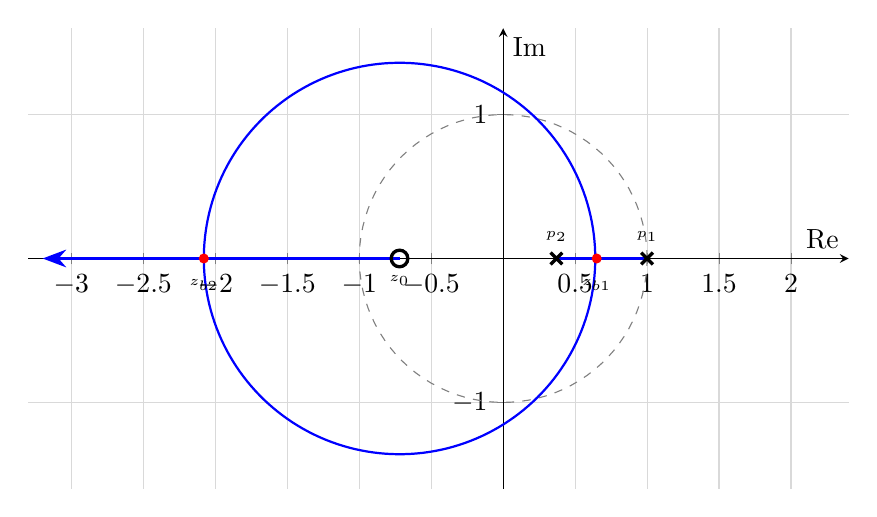
\begin{tikzpicture}
\begin{axis}[
  width=12cm,height=9cm,
  xlabel={$\mathrm{Re}$}, ylabel={$\mathrm{Im}$},
  xmin=-3.3,xmax=2.4,ymin=-1.6,ymax=1.6,
  axis equal image,
  axis lines=middle,
  grid=both, minor grid style={gray!15}, major grid style={gray!30},
]
\addplot[gray,dashed,domain=0:360,samples=100] ({cos(x)},{sin(x)});
\addplot[blue,thick,domain=0:360,samples=200] ({-0.72+1.36*cos(x)},{1.36*sin(x)});
\addplot[blue,thick] coordinates {(0.37,0)(0.65,0)};
\addplot[blue,thick] coordinates {(0.65,0)(1,0)};
\addplot[blue,thick] coordinates {(-2.08,0)(-0.72,0)};
\addplot[blue,thick,-{Stealth[length=3mm]}] coordinates {(-2.08,0)(-3.2,0)};
\addplot[only marks,mark=x,black,mark size=3pt,line width=1.2pt] coordinates {(1,0)(0.37,0)};
\addplot[only marks,mark=o,black,mark size=3pt,line width=1.2pt] coordinates {(-0.72,0)};
\addplot[only marks,mark=*,red,mark size=1.6pt] coordinates {(0.65,0)(-2.08,0)};
\node[above] at (axis cs:1,0.05) {\tiny $p_1$};
\node[above] at (axis cs:0.37,0.05) {\tiny $p_2$};
\node[below] at (axis cs:-0.72,-0.05) {\tiny $z_0$};
\node[below] at (axis cs:0.65,-0.08) {\tiny $z_{b1}$};
\node[below] at (axis cs:-2.08,-0.08) {\tiny $z_{b2}$};
\end{axis}
\end{tikzpicture}
\end{center}
(cerc punctat = cerc unitate.)

\section*{Teorie (pe scurt)}

\subsection*{1. Transformarea $s\to z$ (porțiunea 5-6)}
$$\color{blue}z=e^{sT_e}:\quad \mathrm{Re}(s)=0\to|z|=1;\quad \mathrm{Re}(s)<0\to|z|<1\quad\Rightarrow\text{aliasing}$$

\subsection*{2. Frecvența de eșantionare (aliasing)}
$$\color{blue}\omega_e>2\omega_{max}\qquad(\text{Nyquist--Shannon})$$

\subsection*{3. Etapele conversiei A/N}
$$\color{blue}\text{Eșantionare}\to\text{Reținere (S\&H)}\to\text{Cuantizare}\to\text{Codificare}$$

\subsection*{4. Eșantionare + reconstrucție cu ERO}
$$\color{blue}x^*(t)=\sum_{k=0}^\infty x(kT_e)\,\delta(t-kT_e)\qquad \hat x(t)=x(kT_e),\ kT_e\le t<(k+1)T_e\qquad G_{ERO}(s)=\frac{1-e^{-sT_e}}s$$
\begin{center}
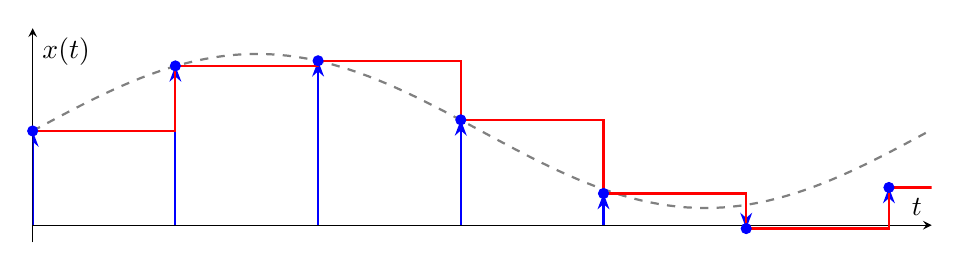
\begin{tikzpicture}[scale=1,>=Stealth]
\begin{axis}[
  width=13cm,height=4.3cm,
  xlabel={$t$}, ylabel={$x(t)$},
  xmin=0,xmax=6.3,ymin=-0.2,ymax=2.3,
  axis lines=middle,
  ytick=\empty, xtick=\empty,
  grid=none,
]
\addplot[gray,thick,domain=0:6.3,samples=100,dashed] {1.1+0.9*sin(deg(x))};
\addplot[only marks,mark=*,blue,mark size=1.8pt] coordinates {
(0,1.1)(1,1.86)(2,1.92)(3,1.23)(4,0.37)(5,-0.04)(6,0.44)
};
\draw[blue,thick,-{Stealth[length=2mm]}] (0,0) -- (0,1.1);
\draw[blue,thick,-{Stealth[length=2mm]}] (1,0) -- (1,1.86);
\draw[blue,thick,-{Stealth[length=2mm]}] (2,0) -- (2,1.92);
\draw[blue,thick,-{Stealth[length=2mm]}] (3,0) -- (3,1.23);
\draw[blue,thick,-{Stealth[length=2mm]}] (4,0) -- (4,0.37);
\draw[blue,thick,-{Stealth[length=2mm]}] (5,0) -- (5,-0.04);
\draw[blue,thick,-{Stealth[length=2mm]}] (6,0) -- (6,0.44);
\addplot[red,thick,const plot mark left] coordinates {
(0,1.1)(1,1.86)(2,1.92)(3,1.23)(4,0.37)(5,-0.04)(6,0.44)(6.3,0.44)
};
\end{axis}
\end{tikzpicture}
\end{center}
(gri = $x(t)$; săgeți = $x^*(t)$; roșu = $\hat x(t)$ reconstruit cu ERO.)

\end{document}
